\subsubsection{Addition Operator}

The test takes 10 million positive randomly generated integers and calculates the sum of them. See Figure \ref{fig:net_addition} for results. Other operators such as subtraction, multiplication, division and modulo were also tested but generated the same results except in the case of Python where they were all slower due to the sum function being more efficient than the reduce function.

\begin{figure}[h]
	\centering
	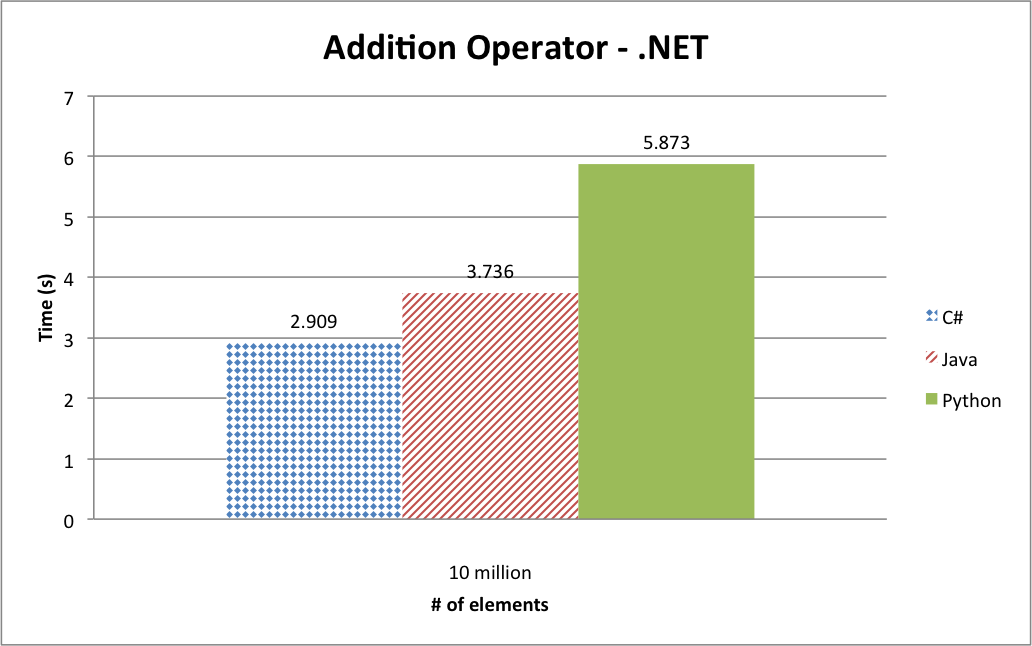
\includegraphics[width=1.0\linewidth]{chapters/new_media/AdditionOperatorNet.png}
	\caption{This tests a language ability to sum 10 million elements. Lower is better. The results show that C\# running in its native environment (.NET) is the fastest of the three languages with 2.909 seconds. Python is the slowest of the three with a runtime of 4.867 seconds.}
	\label{fig:net_addition}
\end{figure}
